\section{Interaction Model}
\label{sec:interface}

% In the semi-autonomous vehicles we introduced in the previous section,
% a human driver can always intervene and simply follow the traffic
% signal.

% , as long as no driver runs a red light (without a
% reservation granted).

Safety is a main concern when involving human drivers in the control
loop of semi-autonomous vehicles.  For the semi-autonomous vehicles
defined above to be able to go through an intersection safely, we need
to define a simple and clean interface for negotiating with the IM and
passing control between the human driver and the driver agent.  In
this section, we describe how our proposed protocol can be realized
safely by having an \emph{interaction model} between human drivers and
driver agents that simplifies the task of the human drivers.

Figure~\ref{fig:interaction} summarizes the interaction model between
human drivers, driver agents, and the IM.  We require the inclusion in
the vehicle of a single button that signals the driver agent to ask
for a reservation. After pressing the button, the driver agent will
automatically send a request message to the IM on behalf of the human
driver. It is also important that there is a clear ``Okay'' indicator
(such as a green light) installed in the car which indicates when the
request has been confirmed.  After seeing the okay signal, the driver
would have to actively pass control to the driver agent, again by
pressing a single button.  This way the driver will not be surprised
by any sudden autonomous actions of the vehicle.

\begin{figure*}[t]
\centering
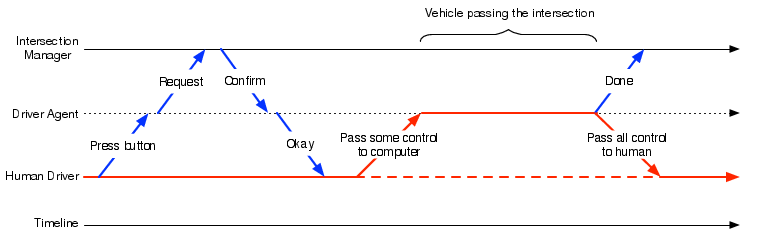
\includegraphics[width=5.5in]{figures/interaction}
\caption{The interaction between human drivers, driver agents, and the
IM.  The blue lines are message passing, and the read lines are
transfer of control.  Note that human drivers retain some control of the vehicle
inside the intersection (the dashed red line).}
\label{fig:interaction}
\end{figure*}

Keep in mind that the only thing a human driver needs to do is to
first press a single button to request a reservation and then press a
single button to accept it (possibly the same button).  All of the
negotiation involving arrival times and trajectories is completed
automatically by the driver agent and IM in a manner similar to how it
is done in AIM.  

Moreover, before entering the intersection the human driver can still
choose to \emph{opt out} without entering the intersection.  All he or she 
needs to do is to touch the brakes and stop before the
intersection.~\footnote{More precisely, if a human driver chooses to
opt out, he must touch the brake before the \emph{point of no return}
beyond which it would be too late for the vehicle to stop.  The
position of the point of no return depends on the speed of the
vehicle.}  The human driver will regain control, and then have to
drive as done today and respect the traffic signals even if they
have gotten a confirmation from the IM.

After passing control to the driver agent, the human driver still
needs to maintain limited control of the vehicle because the vehicle
is not fully autonomous.  The question of how to achieve this
human-computer cooperative driving depends on the type of
semi-autonomous vehicle as well as the type of intersection.  In
case of Type SA-ACC vehicles, the human driver must keep following the
vehicle ahead by steering the vehicle in the correct direction.  At
intersections where the vehicle ahead must make a sharp turn, the IM
would deny the reservation to the vehicle.  In the case of SA-CC
vehicles, the human driver simply holds the steering wheel to make the
vehicle goes straight through the intersection.  In Type SA-Com
vehicles, no control is passed to the driver agent, and the IM will
reserve the entire lane for the vehicle for a period of time.  The
human driver has to make sure that the vehicle goes through the
intersection within that period of time, perhaps with the help of a
virtual traffic signal on the computer screen.

This interaction model only requires the human driver to perform
relatively simple driving maneuvers such as holding the steering wheel
at a certain angle (for Types SA-ACC and SA-CC vehicles) or
driving as if under a traffic signal (for Type SA-Com vehicles).
These tasks are much simpler than other maneuvers such as lane
changing and passing other vehicles, and thus should not be taxing to experienced human drivers.  
%Thus it is reasonable to assume
%that human drivers, with enough practice, should manage to perform
%these maneuver perfectly.

% There is a point near the entry of the intersection where it is no
% longer possible to brake before entering the intersection. Beyond this
% point, the person must lose the ability to take back control of the
% speed until leaving the intersection (presumably with an emergency
% override option for extreme situations).  This constraint is based on
% the fact that if the driver were to change its velocity, its
% reservation would need to be modified.  The IM cannot guarantee that
% the modified reservation will be confirmed.

% If the person touches the brakes or accelerator, the person
% regains control, and the reservation is cancelled.


% Two points are important to keep in mind about all the cases above:
% \begin{itemize}
% \item The only actions a human driver needs to take is to press a
% single button to request a reservation, and press a single button to
% accept it (possibly the same button).  All of the negotiation
% involving arrival times and trajectories is completed automatically by
% the driver agent and IM in a manner similar to how it is done in AIM.
% \item No equipment is \emph{required} on any car.  Like FCFS-Signal in
% AIM, SemiAIM is fully compatible with ``classic'' human-driven cars
% that have no communications equipment.
% \end{itemize}




% Drivers can must always steer in type SA-CC vehicles. For type SA-ACC,
% the vehicle might follow a vehicle in front of it to make a turn. The
% driver would cede control over the steering wheel in this case.

% If the request is confirmed and the
% driver decides not to enter, it still does no harm (even though the
% tiles it requested are wasted).  When the reservation is granted to
% Types SA-ACC and SA-CC vehicles, the vehicle starts controlling the
% speed.



% \commentp{It would be useful in this section to add a flowchart or
% some other representation of how and when control passes between the
% car and the person.}

% \section{Definitions}

% A road $r$ consists a finite number of lanes $l_1$, $l_2$, \ldots,
% $l_n$.  We write $r = (1_1, l_2, \ldots l_n)$.
% All lanes in a road are in the same direction.
% An \emph{entry} road of an intersection is a road
% from which traffic flows into the intersection.
% An \emph{exit} road is a road from which traffic flows out of
% an intersection.


% \section{A General AIM architecture}

% We generalize the AIM architecture as follows.

% \commentc{Maybe draw a diagram to show to how AIM works}

% This framework can be considered as an extension to AIM.
% In AIM, each request is a $4$-tuple $\langle t, v, l_1, l_2 \rangle$.
% \commentc{Fit AIM requests into the next framework.}

% In AIM, these values are *exact*. However, in SemiAIM,
% these values can be constrained.

% No need to think about the acceleration schedule yet.

% In essence, no human intervention is involved in the control loop.


%%% Local Variables: 
%%% mode: latex
%%% TeX-master: "main"
%%% End:
